%Started on Friday, 11 August 2006
%Aug: 23, 29, 30, 31
%Sep:  1
% 2007
%Jan: 16, 17, 22
%Feb:  6,  9, 11, 22
%Mar:  8, 20

%
% Chapter: 
%
\label{ch:Correctors}

In this chapter we illustrate the theoretical understanding of 
the cases of failure of Mehrotra's corrector direction,
drawing particularly from \cite{Cartis04,Cartis05}.
We discuss subspace searches as a way to determine good
search directions, and present a computationally competitive way
to improve the performance of multiple centrality correctors.
The original content of this chapter has already appeared 
in \cite{ColomboGondzio05}, co-authored with Jacek Gondzio.


%
% Section
%
\section{Weaknesses in the existing approaches}

Newton's method applied to the primal--dual path-following algorithm 
provides a first-order approximation of the central path, in which
the nonlinear KKT system (\ref{eq:PerturbedKKT}) corresponding 
to the barrier problem 
is linearised around the current point $(x^k,y^k,s^k)$. Consistently with 
the standard analysis of Newton's method, this linear approximation 
is valid locally, in a small neighbourhood of the point where 
it is computed. Depending on the specific characteristics of the point, 
such an approximation may not be a good direction at all 
if used outside this neighbourhood.

Mehrotra's algorithm, as already discussed in 
Section~\ref{sec:MehrotraPC}, adds a second-order correction to the search 
direction in order to construct a quadratic approximation 
of the central path. This technique is at the basis of all
implementations of interior point methods for linear programming,
and the practical superiority of a second-order algorithm over 
a first-order one is broadly recognised.
However, the central path is a highly nonlinear curve that, according 
to Vavasis and Ye \cite{VavasisYe}, is composed by $O(n^2)$ turns 
of a high degree and segments in which it is approximately straight. 
Given the complexity of this curve, it is unrealistic to be able 
to approximate it everywhere with a second-order curve.

\ignore{
In particular, as was noted by
Mehrotra himself \cite{Mehrotra92}, the main advantage comes from 
the use of the second-order term in the corrector direction.
}

Failures of Mehrotra's corrector have been known by practitioners 
since its introduction. In practical implementations, it was noticed 
that Mehrotra's corrector would sporadically produce a shorter stepsize 
than the one obtained in the predictor direction. 
In such situations, it is common for a solver
to reject the corrector, then try to use some multiple centrality 
correctors or move along the predictor direction alone.

\fb{
Run Netlib problems with HOPDM, print Mehrotra rejected, and count them.
}

This issue has recently been analysed by Cartis \cite{Cartis04}, 
who provided an example in which the second-order corrector does 
not behave well. Cartis's analysis is based on an algorithm 
that combines a standard primal--dual path-following method with 
a second-order correction. Despite not being exactly Mehrotra's 
predictor--corrector algorithm, both are very close in spirit.
Cartis's example shows that for certain starting points the corrector 
is always orders of magnitude larger than the predictor, in both 
primal and dual spaces. Whilst the predictor points towards 
the optimum, the second-order corrector points away from it.
As the final direction is given by
\[
\Delta = \Delta_{a} +\Delta_c,
\]
the combined direction is influenced almost exclusively by the corrector, 
hence it is not accurate. 

\fb{
Where does this misbehaviour come from?

Coralia's starting point is badly centered.
Maybe we could try other points and see if a better centred point fixes
the issue of the large magnitude of the corrector.
}

The solution outlined by Cartis in \cite{Cartis04}, and then further 
developed in \cite{Cartis05}, is to reduce the influence exerted by 
the corrector by weighting it by the square of the stepsize. 

Besides ensuring that the corrector is really considered 
a second-order term as in a rigorous Taylor expansion, 
this proposal allows for better convergence results.

\fb{
Present some results.
}

In a similar way, Salahi et al. \cite{SalahiPengTerlaky} propose to find 
the corrector by weighting the term $\Delta_a X \Delta_a S e$ in 
(\ref{eq:MehrotraRhs}) by the allowed stepsize for the affine-scaling 
direction.

\ignore{
A weakness in Mehrotra's algorithm concerns the computation of the 
second order direction. In this procedure, it is assumed that a 
full step in the affine scaling direction has been taken. This is 
most definitely not the case, as a full step in the affine scaling 
direction would produce the optimal solution. Moreover, while
the real maximum step in the predictor direction is computed, 
in Mehrotra's algorithm this is only used to evaluate the quality 
of the predictor.

Multiple centrality correctors try to fix the presence of outliers in 
complementarity products after the computation of a complete 
predictor--corrector pair. This setup overlooks the fact that the 
presence of outliers is known from the beginning of the iteration. 
Still, in the centrality term,  we ask all of them to align to the 
average $\mu$.
}

A better understanding of these issues and a solution to these
problems will be the major focus of the next sections.


%
% Section
%
\section{Subspace searches}

Subspace searches are a different strategy of generating search 
directions. 
They are usually derived differently than from the Newton system, and 
are built according to some criteria that are believed to be essential 
for a good search direction.

%
%
\subsection{Jarre and Wechs's directions}

Jarre and Wechs \cite{JarreWechs} % took a more pragmatic view and
looked for an implementable technique for generating efficient 
higher-order search directions in a primal--dual interior-point framework.
In the Newton system, while it is clear what to consider as right-hand 
side for primal and dual feasibility constraints (the residual 
at the current point), the complementarity component leaves more 
freedom in choosing a target $t$. They argue that there exists 
an optimal choice for which the corresponding Newton system would 
produce immediately the optimizer; however, it is not obvious how 
to find it.
Therefore, they propose to search a subspace spanned by $k$ different 
directions $\Delta w_1, \Delta w_2, \ldots, \Delta w_k$ generated 
from some affinely independent targets $t_1,t_2,\ldots,t_k$.
As the quality of a search direction can be measured by the length 
of the stepsize and the reduction in complementarity gap, they aim 
to find the combination 
\[
\Delta w = \Delta w(\rho) 
         = \rho_1\Delta w_1 + \rho_2\Delta w_2 + \ldots + \rho_k\Delta w_k
\]
that maximizes these measures.
This can be formulated as a small linear subproblem which can 
be solved approximately to produce a search direction $\Delta w$ 
that is generally better than Mehrotra's predictor--corrector direction.

\fb{
Present analysis from Jarre-Wechs \cite{JarreWechs}.
}

The way they construct the search direction is the following. 
Given the system
\be
\label{eq:JarreWechsSystem}
\left[ \begin{array}{ccc}
    A & 0   & 0 \\
    0 & A^T & I \\
    S & 0   & X
  \end{array} \right]
\left[ \begin{array}{c}
    \Delta x \\ \Delta y \\ \Delta s
  \end{array} \right] =
\left[ \begin{array}{c}
    b-Ax \\ c-A^Ty-s \\ t
  \end{array} \right],
\ee
%where $t=\mu e-XSe$, 
they ask what 
choice of right-hand side $t$ would produce a good search direction.

Let $w=(x,y,s)$ be the current point and 
$w^*=(x^*,y^*,s^*)$ be an optimal primal--dual solution to 
the system (\ref{eq:JarreWechsSystem}).
Therefore $\Delta w^*= w^*-w$ satisfies the 
system when $t=X\Delta s^* + S\Delta x^*=t^*$. Therefore,
this particular choice of $t^*$ proves to be the best overall,
as it leads to the optimizer.

Obviously, when the system is set up, we have no knowledge of 
$t^*$. However, a lower bound can be determined. Knowing that 
$s^*+\Delta s^* \ge 0$ and $x^*+\Delta x^* \ge 0$, we have 
$\Delta s^* \ge -s^*$ and $\Delta x^* \ge -x^*$, from which:
\[
t^*= X\Delta s^* + S\Delta x^* \ge -2XSe.
\]

\fb{
It would be interesting to see if in practice this bound is useful. 
We could check whether at any iteration it's violated, and if so just
put the bound...
}

An upper bound is derived from a result by Vavasis and Ye 
(Lemma~16 in \cite{VavasisYe}):
\begin{quote}
``Let $(x,y,s)$ and $(x',y',s')$ be two points on the central 
path such that $0<\mu'<\mu$. Then, for any $i$:
$s_i' \le ns_i$, and $x_i' \le nx_i$.''
\end{quote}

From this, immediately we obtain that if $(x,s)$ is on the 
central path, then
\[
(\Delta x^*,\Delta s^*)\le(n-1)(x,s).
\]
Considering the final step of the proof in the cited Lemma:
\[
\frac{x_i'}{x_i} +\frac{s_i'}{s_i} \le n,
\]
we can obtain the equivalent expression 
$s_ix_i' + x_is_i' \le nx_is_i$, and so
\[
SX'e + XS'e \le nXSe.
\]
Therefore, we can produce the following upper bound:
\[
t^*= X\Delta s^* +S\Delta x^* = X(s^*-s)+S(x^*-x) = 
     \underbrace{XS^*e + SX^*e}_{\le nXSe} -2XSe \le (n-2) XSe.
\]

It is possible to write $t^*$ as a different expression. 
Given that $X^*S^*e=0$, we have:
\[
0 = (X+\Delta X^*)(S+\Delta S^*)e = XSe + 
    \underbrace{X\Delta s^* +S\Delta x^*}_{=r^*} +\Delta X^*\Delta S^*e,
\]
from which $t^* = -XSe - \Delta X^* \Delta S^*e$.

They consider how to use Mehrotra's corrector in an iterative 
fashion, and notice that a straightforward recursion of the type
\begin{eqnarray*}
  A\Delta x^j &=& b-Ax \\
  A^T\Delta y^j +\Delta s^j &=& c-A^Ty-s \\
  X\Delta s^j + S\Delta x^j &=& \mu e  -XSe -\Delta X^{j-1}\Delta S^{j-1}e
\end{eqnarray*}
is usually divergent for general positive starting points.

\fb{
They noticed that following targets generated by iterating Mehrotra's 
corrector in a straightforward recursion of the type
\[
t^{k+1} = \mu e - XSe - \Delta X^k\Delta S^k e
\]
usually shows a divergent behaviour for general positive starting 
points. Therefore, they introduce a rescaling of Mehrotra's corrector 
and other strategies to guarantee good convergence properties.
}

%
%
\subsection{Krylov subspace searches}

While the multiple centrality correctors approach 
presented in Section~\ref{sec:MultipleCC} 
generates a series of correctors 
that are evaluated and applied recursively, Mehrotra and Li 
\cite{MehrotraLi} propose a scheme in which a collection of linearly 
independent directions is combined through a small linear subproblem.

Following the approach explored by Jarre and Wechs \cite{JarreWechs}, 
they express the requirements for a good search direction as a linear 
program. In particular, they impose conditions aimed at ensuring 
global convergence of the algorithm when using generic search directions.
The directions considered in the subspace search can include all 
sorts of linearly independent directions: affine-scaling direction, 
Mehrotra's corrector, multiple centrality correctors, Jarre--Wechs 
directions. 
In their approach, Mehrotra and Li \cite{MehrotraLi}
generate directions using a Krylov subspace mechanism.

% This new approach for generating corrector directions uses an exact 
% factorization from an earlier iteration to generate directions 
% via Krylov subspaces. 
% Therefore, information obtained from an iterative scheme is used 
% to improve the performance of an implementation based on direct 
% methods. In some sense, it is a hybrid of direct and iterative methods.

% When generating correctors through Krylov subspaces, the directions 
% have to satisfy the primal--dual feasibility constraints, but not 
% the complementarity constraints. This means that any convex combination 
% of these directions will still satisfy the feasibility requirements; 
% this gives the additional freedom of choosing the combination that 
% satisfies the complementarity conditions in the best possible way. 
% {\bf (Note: M\&L don't require the linear combination to be convex.)}

At the $k$-th iteration of interior point method we have to solve 
the Newton system $H_k \Delta_k = \xi_k$, where 
\[
\xi_k = 
%\left[
%  \begin{array}{c}
%    \xi_p \\
%    \xi_d \\
%    \xi_{\mu} 
%  \end{array}
%  \right] =
\left[
  \begin{array}{c}
    b - A x^k \\
    c - A^T y^k - s^k \\
    \mu e - X^k S^k e 
  \end{array}
  \right]
\]
is the right-hand side evaluated at the current iterate and $H_k$ 
is the corresponding Jacobian matrix. 
%
The direction $\Delta_k$ is used to compute a trial point:
\[
\tilde{x} = x^k + \alpha_P \Delta_k x, \quad
\tilde{y} = y^k + \alpha_D \Delta_k y, \quad
\tilde{s} = s^k + \alpha_D \Delta_k s.
\]
%
At the trial point $(\tilde x, \tilde y, \tilde s)$, a usual 
interior point method would have to solve the system
$\tilde H \tilde \Delta = \tilde \xi$
in order to find the next search direction. Instead, 
Mehrotra and Li \cite{MehrotraLi} generate a Krylov subspace 
for $\tilde H \tilde \Delta = \tilde \xi$.
The Krylov subspace of dimension $j$ is defined as
\[
K_j (H_k, \tilde H, \, \tilde \xi) =
{\mbox{span}} \{ \xi_H, G \xi_H, G^2 \xi_H, \dots,  G^{j-1} \xi_H \}, 
\]
where $\xi_H = H_k^{-1} \tilde \xi$, and $G = I - H_k^{-1} \tilde H$. 
Note that for stability reasons $\tilde H$ is preconditioned with $H_k$, 
the factors of which have already been computed.
The subspace thus generated contains $j$ linearly independent directions. 

In the algorithm of \cite{MehrotraLi}, the affine-scaling
direction $\Delta_a$, Mehrotra's corrector $\Delta_0$, 
the first $j$ directions $\Delta_1, \Delta_2, \dots, \Delta_j$ 
from $K_j (H_k, \tilde H, \tilde \xi)$ and, but only under some 
circumstances, a pure recentering direction $\Delta_{cen}$ are 
combined with appropriate weights $\rho$:
\[
\Delta(\rho) = \rho_a\Delta_a + \sum_{i=0}^j \rho_i \Delta_i 
             + \rho_{cen}\Delta_{cen}.
\]
The choice of the best set of weights $\rho$ in the combined search 
direction is obtained by solving an auxiliary linear programming 
subproblem. The subproblem maximizes the rate of decrease 
in duality gap whilst satisfying a series of requirements:
non-negativity of the new iterate,
upper bounds on the magnitude of the search direction,
upper bounds on infeasibilities,
decrease in the average complementarity gap,
and closeness to the central path.

%Both the theoretical formulation and the computer implementation 
%allow for the independent choice of weights $\rho$ for the primal 
%and dual spaces.


%
% Section
%
\section{A practical implementation}

\fb{
Connect better with the previous section.
}

The theoretical findings 
outlined above give rise to the following generalisation
\[
\Delta = \Delta_{a} +\omega\Delta_c,
\]
where we weight the corrector by a parameter $\omega\in(0,1]$ 
independent of $\alpha$.

In our implementation the weight is chosen independently at each 
iteration such that the stepsize in the composite direction 
is maximized. This gives us the freedom to find the optimal weight 
$\hat\omega$ in the interval $(0,1]$. 
%Therefore, we are not committed to using a full weight throughout.
%
This generalisation allows for the possibility of using Mehrotra's 
corrector with a small weight, if that helps in producing a better
stepsize; on the other hand, 
the choice $\hat\omega=1$ yields Mehrotra's corrector again. 
%  On the other hand, $\omega=\alpha$ produces the algorithm 
%  suggested by Salahi~{\em et al.} \cite{SalahiPengTerlaky}.

\fb{
Discuss the difficulties related to the choice of $\omega$.
}

%
%
\subsection{Extension to multiple centrality correctors}

We have applied the weighting strategy to multiple centrality correctors 
as well. The justification in this case comes from the following argument.
In Section~\ref{sec:MultipleCC} we have seen that the target point 
in the multiple centrality correctors technique depends on the
aspiration level
$\delta$ which measures the greediness of the centrality corrector. 

In the previous implementations, this parameter was fixed at coding time 
to a value determined after tuning to a series of representative 
test problems. However, for a specific problem such a value may be 
too conservative or too aggressive; moreover, the same value may not 
be optimal throughout the solution of the same problem. 
Hence, it makes sense to provide 
a mechanism that changes these correctors adaptively in order 
to increase their effectiveness.

\fb{
Maybe present a table where for a subset of problems we show the 
the value of the stepsizes for a fixed $\delta$ and for an
adaptive $\delta\omega$.
}

In our implementation we generate a sequence of multiple centrality 
correctors, and for each of them we choose the optimal weight 
$\hat \omega$ which maximizes the stepsizes in primal and dual spaces 
for a combined direction of the form
\[
  \Delta = \Delta_p + \omega \Delta_c.
\]
The composite direction $\Delta = \Delta_p + \hat \omega \Delta_c$ becomes
a predictor for the next centrality corrector, hence the correcting process
is recursive, and can be interrupted at any stage.

Below we formalise the weighted correctors algorithm.
\begin{description}
\item[Given] an initial iterate $(x^0,y^0,s^0)$ such that $(x^0, s^0) > 0$;
\item[Repeat] for $k=0,1,2,\ldots$ until some convergence criteria are met:
  \begin{itemize}
  \item Solve system (\ref{eq:NewtonSystem}) with right-hand side $r_1$
        (\ref{eq:PredictorRhs}) for a predictor direction $\Delta_a$.

  \item Set $\mu$ according to (\ref{eq:Mu}) and find Mehrotra's corrector 
        direction $\Delta_c$ by solving system (\ref{eq:NewtonSystem}) 
        with right-hand side (\ref{eq:MehrotraRhs}).

  \item Do a linesearch to find the optimal $\hat\omega$ that maximizes 
        the stepsize $\alpha$ in $\Delta^\omega = \Delta_a +\omega\Delta_c$.

  \item Set $\Delta_p = \Delta_a +\hat\omega\Delta_c$. 
    \begin{description}
    \item[Do]
      \begin{itemize}
      \item Solve system (\ref{eq:NewtonSystem}) with right-hand side
	$(0,0,t)$, $t$ given by (\ref{eq:Target}) for a centrality corrector
	direction $\Delta_m$.
      \item Perform a linesearch to find the optimal $\hat\omega$ that maximizes 
        the stepsize $\alpha$ in $\Delta^\omega = \Delta_p +\omega\Delta_m$.
      \item Set $\Delta_p := \Delta_p +\hat\omega\Delta_m$. 
	\end{itemize}
    \item[While] the stepsize increases by at least a fraction of the aspiration level $\delta$;
    \end{description}
  \item Update the iterate $(x^{k+1},y^{k+1},s^{k+1}) = (x^k,y^k,s^k) + \alpha_k\Delta_p (x^k,y^k,s^k).$
  \end{itemize}
\item[End]
\end{description}

%
%
\subsection{Finding an appropriate weight}

Concerning the choice of $\omega$, we implemented a linesearch in
the interval $[\omega_{\min},\omega_{\max}]=[\alpha_P\alpha_D, 1]$. 
There are two reasons for using  $\omega_{\min} = \alpha_P\alpha_D$. 
First, using the stepsizes $\alpha_P$ and $\alpha_D$ for the predictor
direction gives 
\[
(X + \alpha_P \Delta X) (S + \alpha_D \Delta S) e 
\;=\; XSe + \alpha_P S\Delta Xe + \alpha_D X\Delta Se 
          + \alpha_P\alpha_D \Delta X\Delta S e,
\]
and the term $\alpha_P\alpha_D$ appears with the second-order error. 
Secondly, the study of Cartis \cite{Cartis04} suggests squaring 
the stepsize for the corrector. Our computational experience indicates 
that the straight use of $\omega = \omega_{\min} = \alpha_P\alpha_D$
is too conservative. Still, such $\omega_{\min}$ is a reliable lower 
bound for attractive weights $\omega$. 

\fb{
Show a table or a figure for this.
}

The ultimate objective in choosing $\omega$ is to increase the stepsizes 
$\alpha_P$ and $\alpha_D$. These stepsizes depend on $\omega$ 
in a complex way. Examples corresponding to a common behaviour 
are given in Figure~\ref{fig:alphaomega}, where we show how the
product $\alpha_P\alpha_D$
varies depending on the choice of $\omega$ for Mehrotra's corrector at 
two different iterations of problem {\tt capri} of the Netlib collection.
On the left, $\omega \in [0.4, 1]$ and $\hat\omega=0.475$ gives a product
$\alpha_P\alpha_D=0.583$, better than a value of 0.477 that would have
been obtained by using a full weight on Mehrotra's corrector.
On the right, $\omega \in [0.178, 1]$ and the choice of 
$\omega \in (0.6, 0.7)$ leads to the best 
product $\alpha_P\alpha_D$ of about 0.375.
%
\begin{figure}[ht]
  \vspace{-3ex}
  \hspace{-3em}
  \begin{minipage}[t]{0.54\textwidth}
  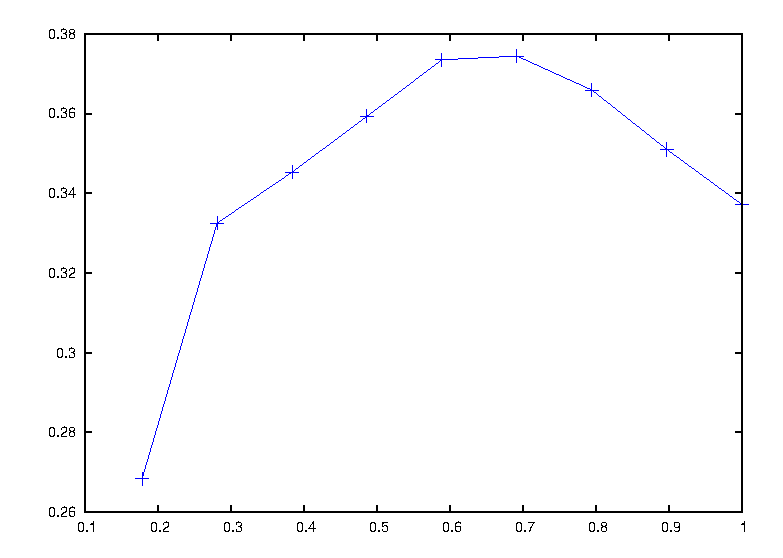
\includegraphics[width=0.73\textwidth,angle=-90]{figures/alphaomega-1.eps}
  \end{minipage} 
  \hspace{-2em}
  \begin{minipage}[t]{0.54\textwidth}
  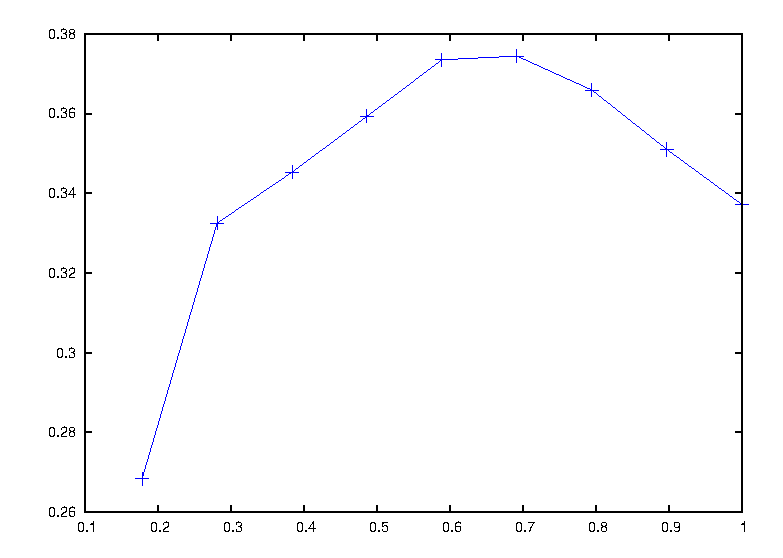
\includegraphics[width=0.73\textwidth,angle=-90]{figures/alphaomega-2.eps}
  \end{minipage}
  \caption{Relationship between $\omega$ and $\alpha_P\alpha_D$ in two iterations of problem {\tt capri}.}
  \label{fig:alphaomega}
\end{figure}

In our crude linesearch procedure we choose 9 points uniformly 
distributed in the interval $[\alpha_P\alpha_D, 1]$ 
and evaluate, for each of these points, the stepsizes in both spaces. 
When a larger stepsize $\alpha_P$ or $\alpha_D$ is obtained, 
the corresponding $\omega$ is stored as $\omega_P$ or $\omega_D$ 
respectively. Hence, we allow two different weightings for directions 
in the primal and dual spaces.

%
% Section
%
\section{Numerical results}
\label{NumRes}

We have implemented our proposal within the HOPDM interior point solver 
\cite{HOPDM}. 
%
%Unlike Mehrotra and Li's approach, which generates Krylov directions and
%chooses weights and combines them into a composite direction, we
%generate a sequence of multiple centrality correctors.
%
We tested our implementation in a series of computational 
experiments, using test problems from different collections. 
As a comparison, we present the results obtained by PCx \cite{PCx}, 
a reference implementation of interior point methods. Since the two 
implementations, PCx and HOPDM, have different termination criteria 
in their default configurations, for the purpose of consistency 
we decided to implement in HOPDM the criteria used in the study 
performed by Mehrotra and Li \cite{MehrotraLi}.
Therefore, optimal termination occurs when the following conditions
are met:
%
\be \label{TermCriteria}
\frac{\mu}{1+|c^T x|} \le 10^{-10}, \qquad
\frac{\|b-Ax\|}{1+\|b\|} \le 10^{-8},  \qquad
\frac{\|c-A^Ty-s\|}{1+\|c\|} \le 10^{-8}.
\ee

\fb{
Criticize these criteria.
}

We use $\gamma = 0.1$ in the definition of symmetric 
neighbourhood and define aspiration levels for the stepsizes using the rule
\[
  \tilde{\alpha}_{P} = \min(1.5 \alpha_{P} \! + \! 0.3, \, 1) 
  \quad \mbox{ and } \quad
  \tilde{\alpha}_{D} = \min(1.5 \alpha_{D} \! + \! 0.3, \, 1). 
\]
The values suggested in \cite{Gondzio96} were more conservative:
$\tilde{\alpha} = \min (\alpha + 0.1, \, 1)$.
Thanks to the weighting mechanism we can control 
the contribution of the corrector in an adaptive way,
and thus be more demanding in the definition of the aspired stepsizes.

Centrality correctors are accepted in the primal and/or dual space
if ${\alpha}_{P}^{new} \geq 1.01 \alpha_{P}$ 
and/or ${\alpha}_{D}^{new} \geq 1.01 \alpha_{D}$, respectively.

\fb{
Note that this is different from what described in \cite{Gondzio96}: there, 
a corrector is accepted if ${\alpha}^{new} \geq \alpha + \gamma\delta_\alpha$, 
where $\gamma = \delta_\alpha = 0.1$. What did HOPDM use to do?
}

We present our results in terms of number of iterations and number 
of backsolve operations. The rationale behind this decision is that 
the multiple centrality correctors technique determines the number 
of allowed correctors on the basis of the ratio between factorization 
cost and backsolve cost. This ratio can be very different across 
implementations, and is mainly influenced by the linear algebra 
routines used. 
HOPDM comes with an in-house linear algebra implementation, while
PCx relies on the more sophisticated sparse Cholesky solver
of Ng and Peyton. Therefore, the PCx code tends to use less 
correctors per iteration.

%
%
\subsection{Mehrotra-Li test collection}
\label{ML-tests}

First we considered the test set used in \cite{MehrotraLi}: 
it contains 101 problems from both Netlib and Kennington collections. 
%
In Table~\ref{MLtotals} we present the computational comparison 
outlining the total number of iterations and the total number 
of backsolves necessary to solve the problems in Mehrotra and Li's test set. 
Column HO displays the results obtained
by the previous implementation, while column dHO reports
the results obtained by the current implementation of weighted
correctors with a default choice of the number of centrality correctors. 
The last column presents the relative change between the two 
versions of HOPDM tested. 
As a reference, we also report in this table the overall
statistics of PCx (release 1.1) on these problems. Also for PCx we adopted
the termination criteria (\ref{TermCriteria}).
We found the number of backsolves by counting the number of calls 
to the functions {\tt IRSOLV()} and {\tt EnhanceSolve()}, for HOPDM and
PCx respectively.
%
\begin{table}[ht]
  \centering
  \begin{tabular}{|l|c||c|c|r|}\cline{2-5}
    \multicolumn{1}{c|}{}& PCx & HO & dHO &\multicolumn{1}{c|}{Change}\\ \hline
    Iterations       & 2114 & 1871  & 1445           &   -22.77\% \\ 
    Backsolves       & 4849 & 6043  & 5717           &   -5.39\%  \\
    Backsolves/iter. & 2.29 & 3.23  & 3.95           &   +22.29\% \\ \hline
  \end{tabular}
  \caption{Overall results obtained on Mehrotra and Li's test collection.}
  \label{MLtotals}
\end{table}
%
\\From Table~\ref{MLtotals} we first observe the very small number 
of backsolves per iteration needed by PCx. This is due to the fact 
that PCx allows the use of Gondzio's multiple centrality correctors 
only in 4 problems: {\tt dfl001}, {\tt maros-r7}, {\tt pds-10} and 
{\tt pds-20}.
%
Also we notice that when we allow an adaptive weighting 
of the correctors there is a tendency to use more correctors 
per iteration than previously. 
This happens because the weighting mechanism makes it more likely
to accept some correctors that otherwise would have been rejected
as too aggressive.
While this usually leads to a decrease 
in iteration count, it also makes each iteration more expensive.

In Table~\ref{TimeML} we detail the problems for which we obtained savings 
in computational time. Given the small dimension of most of the problems 
in the Netlib collection, we did not expect major savings. However, as the
problem sizes increase, we can see that the proposed way of evaluating and
weighting the correctors pays off. This led us to investigate further 
the performance of the proposed implementation, which we will discuss
in Section~\ref{BN-tests}.
%
\begin{table}[ht]
  \centering
  \begin{minipage}[t]{0.36\textwidth}
    \begin{tabular}{|l|r|r|}\hline
      Problem & \multicolumn{1}{c|}{HO} & dHO \\ \hline
      bnl1    &   0.36 &   0.25 \\
      d{f}l001& 150.63 & 114.80 \\
      maros-r7&   7.76 &   7.52 \\
      pilot   &   5.23 &   4.35 \\ \hline
    \end{tabular}
  \end{minipage}
  \begin{minipage}[t]{0.36\textwidth}
    \begin{tabular}{|l|r|r|}\hline
      Problem & \multicolumn{1}{c|}{HO} & dHO\\ \hline
      pilot87 &  12.62 &  11.88 \\ 
      pds-06  &  24.59 &  21.31 \\
      pds-10  &  96.57 &  79.29 \\
      pds-20  & 923.71 & 633.64 \\ \hline
    \end{tabular}
  \end{minipage}
  \caption{Problems that showed time savings (times are in seconds).}
  \label{TimeML}
\end{table}

We were particularly interested in comparing the results produced by our 
weighted correctors approach with those published in \cite{MehrotraLi}. 
%A full comparison is presented in Table~\ref{MLresults}.
%In terms of the number of iterations, Mehrotra and Li's scheme is extremely 
%promising. 
% However, only 13 problems out of 101 showed a reduction 
% in computing time when using 4 Krylov directions. 
%
The computation of Krylov subspace directions in Mehrotra and Li's 
approach does involve considerable computational cost, as
%While we recognise that the availability of different directions that
%can be mixed together to form a better combined direction is effective,
the computation of each Krylov direction requires a backsolve operation. 
This can be seen from the definition of the power basis matrix
\[
G = I - H_k^{-1}\tilde H,
\]
which involves an inverse matrix. In fact, calling $u$ the starting vector 
in the Krylov sequence, the computation of the vector $ H_k^{-1}\tilde Hu$ 
requires first to compute $v = \tilde Hu$ (matrix--vector multiplication) 
and then to determine $t=H_k^{-1}v$ (backsolve on the Cholesky factors).

In the tables of results presented in \cite{MehrotraLi}, the best 
performance in terms of iteration count is obtained by PCx4, which 
uses 4 Krylov subspace vectors. These directions are combined with 
an affine-scaling predictor direction and Mehrotra's second-order 
correction, leading to 6 backsolves per iteration. 
%  {\bf (but it's not clear that they use Krylov 
%        directions and solve a linear subproblem at every iteration)}
This number increases when the linear subproblem produces an optimal 
objective value smaller than a specified threshold or the new iterate 
fails to satisfy some neighbourhood condition: in these cases 
the pure centering direction $\Delta_{cen}$ also needs to be computed,
and a seventh backsolve is performed.

As we understand the paper \cite{MehrotraLi}, PCx0 uses exactly 
2 backsolves per iteration: one to compute the affine-scaling direction,
another to compute Mehrotra's corrector; PCx2 and PCx4 compute 
two and four additional Krylov vectors, hence they use
4 and 6 backsolves per iteration, respectively.
In columns HO-0, HO-2 and HO-4, we present 
the results obtained by HOPDM when forcing the use of 0, 2 and 4 
multiple centrality correctors. 
In the column called HO\raisebox{1pt}{-$\infty$} we report the results 
obtained when an unlimited number of correctors is allowed
(in practice we allow no more than 20 correctors).
The last column, labelled dHO, presents the results obtained 
by the default way of choosing the number of correctors allowed.

Consequently, up to 2, 4 and 6 backsolves per iteration are allowed
in PCx0, PCx2 and PCx4 and in HO-0, HO-2 and HO-4 runs, respectively.
The number of backsolves reported for HOPDM includes two needed by 
the initialisation procedure: the number of backsolves 
should not exceed $2 \times {\rm {Its}} + 2$, 
$4 \times {\rm {Its}} + 2$ and $6 \times {\rm {Its}} + 2$ respectively
for HO-0, H0-2 and H0-4.
The observed number of backsolves is often much smaller
than these bounds because the correcting mechanism switches off 
when the stepsizes are equal to 1 or when the corrector does not 
improve the stepsize. Problem {\tt afiro} solved by HO-4 needs 24 
backsolves, 22 of which compute different components of directions, 
hence the average number of backsolves per iteration is only 22/6 
and is much smaller than 6. Occasionally,
as a consequence of numerical errors, certain components 
of direction are rejected on the grounds of insufficient accuracy:
in such case the number of backsolves may exceed the stated upper bounds.
The reader may observe for example that {\tt pilot4} is solved by HO-4
in 16 iterations, but the number of backsolves is equal to 100 and 
exceeds $6 \times 16 + 2 = 98$.

The version HO\raisebox{1pt}{-$\infty$} requires 1139 iterations to solve 
the collection of 101 problems, an average of just above 11 iterations
per problem. This version has only an academic interest, 
yet it reveals a spectacular efficiency of interior point 
methods which can solve difficult linear programs of medium sizes 
(reaching a couple of hundred thousand variables) in just 
a few iterations.
In particular, it suggests that if we had a cheap way of generating
search directions, then it would be beneficial to have as many as possible.

%
%
\subsection{Beyond Netlib}
\label{BN-tests}

We have applied our algorithm to examples from other test collections 
besides Netlib.
These include other medium to large linear programming problems, 
stochastic problems and quadratic programming problems.

We used a collection of medium to large problems taken from different
sources: problems {\tt CH} through {\tt CO9}
are MARKAL (Market Allocation) models; {\tt mod2} through {\tt worldl} are
agricultural models used earlier in \cite{Gondzio96}; problems {\tt route}
through {\tt rlfdual} can be retrieved from 
\begin{center}
{\tt http://www.sztaki.hu/\~{}meszaros/public\_ftp/lptestset/misc/},
\end{center}
problems {\tt neos1} through {\tt fome13} can be retrieved from 
\begin{center}
{\tt ftp://plato.asu.edu/pub/lptestset/}.
\end{center}

In Table~\ref{TimeBN} we detail the sizes of these problems and provide 
a time comparison between our previous implementation (shown in column
HO), and the current one (in column dHO).
This test collection contains problems large enough 
to show a consistent improvement in CPU time: in only 4 problems 
({\tt mod2}, {\tt dbc1}, {\tt watson-1}, {\tt sgpf5y6}) 
we recorded a deterioration of the performance by more than 1 second.
The improvements are significant on problems with a large 
number of nonzero elements. In these cases, dHO
produces savings from about 10\% to 30\%, with the remarkable results
in {\tt rail2586} and {\tt rail4284}, for which the relative savings 
reach 45\% and 65\%, respectively.

More numerical results obtained on some collections of stochastic
programming problems and quadratic problems can be found in
\cite{ColomboGondzio05}.

\begin{small}
\begin{longtable}{|l|rrr|r|r|r|} \hline 
  \multicolumn{1}{|c|}{Problem}
& \multicolumn{1}{c}{Rows}
& \multicolumn{1}{c}{Cols}
& \multicolumn{1}{c|}{Nonzeros}
& \multicolumn{1}{c|}{HO}
& \multicolumn{1}{c|}{dHO}
& \multicolumn{1}{c|}{Change}\\ \hline
\endhead
\hline
\multicolumn{7}{c}{\raisebox{-1ex}{Table~\ref{TimeBN}: Time comparison on 
other large problems (times are in seconds).}}
\endfoot
\label{TimeBN}
CH & 3852 & 5062 & 42910 & 1.03 & 1.23 & 19.4\% \\
GE & 10339 & 11098 & 53763 & 5.72 & 5.46 & -4.5\% \\
NL & 7195 & 9718 & 102570 & 4.37 & 3.95 & -9.6\% \\
BL & 6325 & 8018 & 58607 & 2.15 & 2.14 & -0.5\% \\
BL2 & 6325 & 8018 & 58607 & 2.35 & 2.31 &  -1.7\% \\
UK & 10131 & 14212 & 128341 & 2.48 & 3.21 &  29.4\% \\
CQ5 & 5149 & 7530 & 83564 & 2.54 & 2.60 &  2.4\% \\
CQ9 & 9451 & 13778 & 157598 & 9.67 & 8.84 &  -8.6\% \\
CO5 & 5878 & 7993 & 92788 & 3.16 & 3.59 &  13.6\% \\
CO9 & 10965 & 14851 & 176346 & 21.10 & 15.35 & -27.3\% \\
mod2 & 35664 & 31728 & 220116 & 20.59 & 21.68 & 5.3\% \\
world & 35510 & 32734 & 220748 & 26.35  & 23.41 & -11.2\% \\
world3 & 36266 & 33675 & 224959 & 31.13 & 27.49 & -11.7\% \\
world4 & 52996 & 37557 & 324502 & 73.21 & 56.14 & -23.3\% \\
world6 & 47038 & 32670 & 279024 & 39.33 & 32.79 & -16.6\% \\
world7 & 54807 & 37582 & 333509 & 43.14 & 36.02 & -16.5\% \\
worldl & 49108 & 33345 & 291942 & 43.95 & 36.82 & -16.2\% \\
route & 20894 & 23923 & 210025 & 40.92 & 33.78 & -17.4\% \\
ulevi & 6590 & 44605 & 162207 & 9.04 & 9.55 & 5.6\% \\
ulevimin & 6590 & 44605 & 162207 & 16.52 & 16.46 & -0.4\% \\
%aircraft & 3754 & 7517 & 24034 & 0.28 & 0.32 &  14.3\% \\
dbir1 & 18804 & 27355 & 1067815 & 162.18 & 146.51 & -9.7\% \\
dbir2 & 18906 & 27355 & 1148847 & 208.93 & 156.11 & -25.3\% \\
dbic1 & 43200 & 183235 & 1217046 & 72.96 & 77.31 & 5.9\% \\
pcb1000 & 1565 & 2428 & 22499 & 0.26 & 0.33 & 26.9\% \\
pcb3000 & 3960 & 6810 & 63367 & 1.13 & 1.16 & 2.7\% \\
rlfprim & 58866 & 8052 & 265975 & 15.63 & 15.08 & -3.5\% \\
rlfdual & 8052 & 66918 & 328891 & 71.17 & 49.79 & -30.0\% \\
neos1 & 131581 & 1892 & 468094 & 169.11 & 141.89 & -16.1\% \\
neos2 & 132568 & 1560 & 552596 & 113.86 & 86.13 & -24.4\% \\
neos3 & 132568 & 1560 & 552596 & 132.02 & 120.59 & -8.7\% \\
neos & 479119 & 36786 & 1084461 & 1785.80 & 1386.58 & -22.4\% \\
watson-1 & 201155 & 383927 & 1053564 & 138.60 & 166.21 & 19.9\% \\
sgpf5y6 & 246077 & 308634 & 902275 & 49.58 & 64.45 & 30.0\% \\
stormG2-1000 & 528185 & 1259121 & 4228817 & 1661.54 & 1623.19 & -2.3\% \\
rail507 & 507 & 63009 & 472358 & 9.77 & 10.10 & 3.4\% \\
rail516 & 516 & 47311 & 362207 & 7.59 & 5.89 & -22.4\% \\
rail582 & 582 & 55515 & 457223 & 9.67 & 9.60 & -0.7\% \\
rail2586 & 2586 & 920683 & 8929459 & 1029.36 & 566.82 & -44.9\% \\
rail4284 & 4284 & 1092610 & 12372358 & 2779.63 & 978.48 & -64.8\% \\
fome11 & 12142 & 24460 & 83746 & 407.20 & 265.21 & -34.9\% \\
fome12 & 24284 & 48920 & 167492 & 766.96 & 508.61 & -33.7\% \\
fome13 & 48568 & 97840 & 334984 & 1545.05 & 990.62 & -35.9\% \\
%\hline Totals  & & & & 11537.03  & 7713.8 \\
\end{longtable} 
\end{small}

% The collection of stochastic programming problems contains 119 examples
% and comes from
% \begin{center}
% {\tt http://www.sztaki.hu/\~{}meszaros/public\_ftp/lptestset/stochlp/}. 
% \end{center}
% 
% We have also tested the implementation on a collection of 29 quadratic 
% programming problems, available from
% \begin{center}
% {\tt http://www.sztaki.hu/\~{}meszaros/public\_ftp/qpdata/}.
% \end{center}
%
% Normally, HOPDM automatically chooses between direct and iterative 
% approaches for computing directions. A higher-order correcting scheme
% makes much more sense with the direct approach when 
% backsolve is significantly less expensive than the factorization.
% In order to maintain consistency, we forced HOPDM to use a direct 
% approach when 
% solving this class of problems, rather than an iterative scheme.

%
% Section
%
\subsection{Conclusions}
\label{Conclusions}

In this paper we have revisited the technique of multiple centrality 
correctors \cite{Gondzio96} and added a new degree of freedom to it. 
Instead of computing the corrected direction from 
$\Delta = \Delta_p + \Delta_c$ where $\Delta_p$ and $\Delta_c$ are 
the predictor and corrector terms, we allow a choice of weight 
$\omega \in (0,1]$ for the corrector term and compute 
$\Delta = \Delta_p + \omega \Delta_c$.
We combined this modification with the use of a symmetric neighbourhood
of the central path. We have shown that the use of this neighbourhood
does not cause any loss in the worst-case complexity of the algorithm. 

The computational results presented for different classes of problems 
demonstrate the potential of the new scheme. We have compared our algorithm 
against the recently introduced Krylov subspace scheme \cite{MehrotraLi}.
The two approaches have similarities: they look for a set of attractive 
independent terms from which the final direction is constructed. 
Mehrotra and Li's approach uses the first few elements from the basis
of the Krylov space; our approach generates direction terms using 
centrality correctors of \cite{Gondzio96}. Mehrotra and Li's approach 
solves an auxiliary linear program to find an optimal combination 
of all available direction terms; our approach repeatedly chooses 
the best weight for each newly constructed corrector term (and switches 
off if the use of the corrector does not offer sufficient improvement). 
Eventually, after adding $k$ corrector terms, 
the directions used in our approach have form
\[
\Delta = \Delta_a + \omega_1\Delta_1 + \ldots + \omega_k\Delta_k,
\]
and the affine-scaling term $\Delta_a$ contributes to it without any
reduction. Hence, the larger the stepsize, the more progress we make
towards the optimizer.

The comparison presented in Section~\ref{ML-tests} shows a clear advantage 
of our scheme over that of \cite{MehrotraLi}. Indeed, with the same 
number of direction terms allowed, our scheme outperforms Krylov subspace 
correctors by a wide margin. Multiple centrality correctors show 
consistent excellent performance on other classes of problems
including medium to large scale linear programs beyond the Netlib 
collection and medium scale quadratic programs.

\fb{
Monteiro, Adler and Resende \cite{MonteiroAdlerResende90} talk about
corrector steps.
}


\fb{
It would be good to try and implement using the search direction from
the previous iteration as another (free) direction to span the subspace.
}

\begin{remark}
From the study of subspace searches it is clear that the more 
directions we consider, the better the final search direction 
we get. Therefore, if we had a cheap way of generating search
directions (rather than from solving a system of linear equations),
then these should be employed.
\end{remark}

\begin{remark}
Mehrotra and Li \cite{MehrotraLi} mention employing previous search
directions alongside the usual ones. The use of these incurs an
increased memory usage, but no additional computational cost.
However, it does not seem that they were actually employed in
the runs. This opens some questions on what constitutes a valid
previous direction (only affine scaling, the final composite direction
or something else).
\end{remark}
